\chapter{背景}
\label{chapter:introduction}
\section{两会中的乡村发展}
在中国这片辽阔的土地上,城市的霓虹灯光下掩映着农村的静谧星空。改革开放以来,中国经历了翻天覆地的变化。城市化与工业化的巨轮迅速推进,城乡人口结构发生巨大改变,同时也带来一系列“三农”问题。在这样的背景下,乡村振兴战略的提出成为解决社会主要矛盾的必然需求,是推动城乡协调发展的关键举措。

党的十四届全国人大二次会议中多次提到,推进乡村全面振兴是新时代新征程“三农”工作的总抓手,要锚定建设农业强国目标,学习运用“千万工程”经验,以加快农业农村现代化更好推进中国式现代化建设。要坚持农业农村优先发展,加快现代农业建设,全方位夯实粮食安全根基,多途径促进农民收入较快增长。要坚持农民主体地位,大力培养乡村人才,吸引各类人才投身乡村振兴。要深入推进农村生态文明建设,加快发展方式绿色转型,建设宜居宜业和美乡村。

本文通过爬虫技术梳理了全国两会报告中涉及乡村发展的所有内容,旨在彰显国家对乡村振兴战略的高度重视。
\begin{figure}[H]
    \centering
    \begin{minipage}{0.5\textwidth}
        \centering
        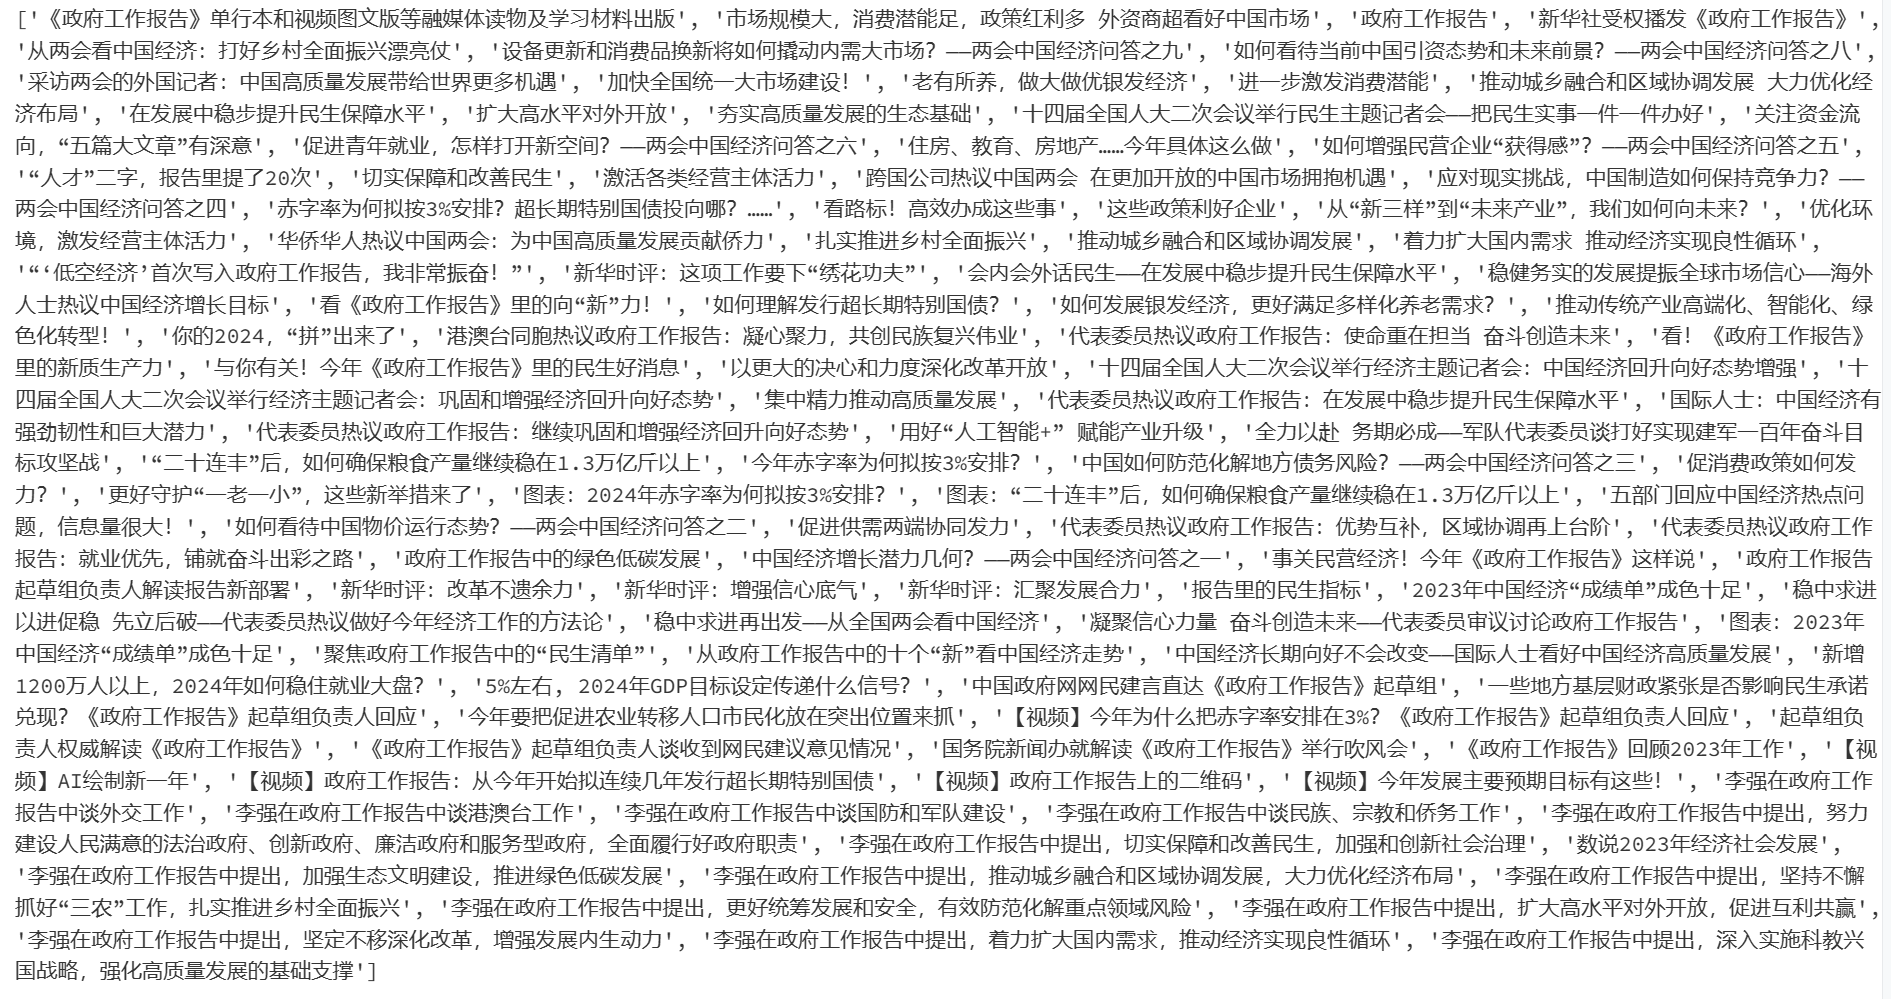
\includegraphics[width=\linewidth]{figures/33.png}
        
        \label{fig:enter-label}
    \end{minipage}\hfill
    \begin{minipage}{0.5\textwidth}
        \centering
        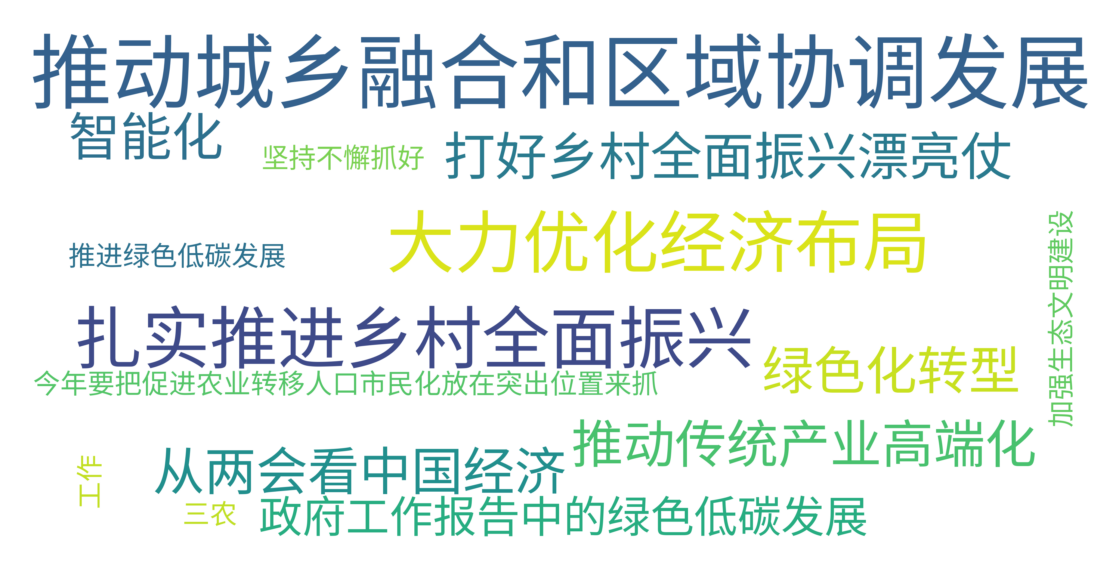
\includegraphics[width=\linewidth]{figures/6.png}
        
        \label{fig:TwoSessions}
    \end{minipage}
    \caption{两会爬虫文本看乡村发展必要性}
\end{figure}

自党的十九大报告首次提出实施乡村振兴战略以来,中国在“三农”工作上已取得了一定成就,本文收集并整理了近年来的相关数据,致力于分析农村发展历程。

\section{角度分析}

在了解到国家高度重视乡村振兴战略的基础上,本文将站在乡村发展的视角上深入探讨这一战略。通过整合《全国乡村产业发展规划(2020-2025年)》的相关文本并筛选出关键词汇,以词云的形式展现本文分析乡村发展的核心内容。

\begin{figure}[H]
    \centering
    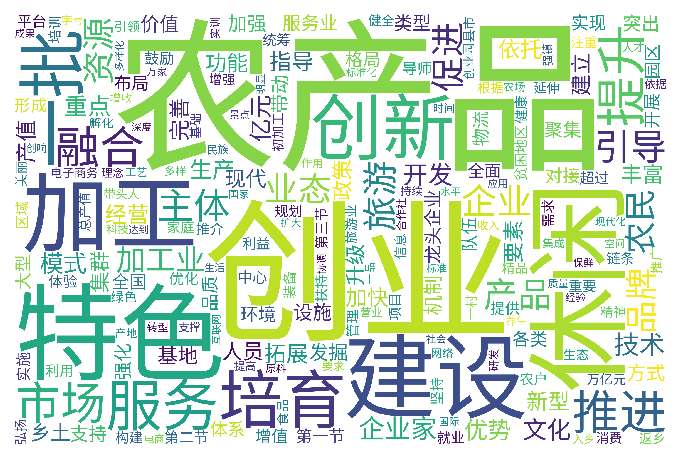
\includegraphics[width=0.6\linewidth]{figures/46.png}
    \caption{全国乡村产业发展规划词云图}
    \label{fig:enter-label}
\end{figure}

在词云中突显出诸多关键词,如“农产品”、“休闲”、“创新创业”、“建设”、“旅游”、“农民”和“就业”等,体现出乡村振兴战略的多维焦点,也为本文后续的论述指明方向。因此,本文将以这些关键词作为基础,解析它们在乡村振兴过程中的具体含义与作用,进而深化对该战略全局性和战术性贯彻落实的认识。